\documentclass[a4paper, 12pt]{article}

%=========
% PACKAGES
%=========

\usepackage{graphicx}
\usepackage[section]{placeins}
\usepackage{float}
\usepackage{amsmath}
\usepackage{listings}
\usepackage{xcolor}
\usepackage{extarrows}
\usepackage{verbatim}
\usepackage{enumerate}
\usepackage{enumitem}
\usepackage{eurosym}
\usepackage{svg}
\usepackage{varwidth}
\usepackage{moreverb}
\usepackage{relsize}
\usepackage{tabto}
\usepackage[margin=1in]{geometry}
\usepackage[normalem]{ulem}
\usepackage{units}
\usepackage{fancyvrb}
\usepackage{fontspec}
\usepackage{extarrows}
\usepackage{amsfonts}
\usepackage{amssymb}
\usepackage{hyperref}
%\usepackage{unicode-math}


%=====================
% SETTINGS/DEFINITIONS
%=====================

% Don't break words with hyphens. Instead, wrap word to next line.
\tolerance=1
% \emergencystretch=\maxdimen
\hyphenpenalty=10000
\hbadness=10000

\definecolor{codegreen}{rgb}{0,0.6,0}
\definecolor{codegray}{rgb}{0.5,0.5,0.5}
\definecolor{codepurple}{rgb}{0.58,0,0.82}
\definecolor{backcolour}{rgb}{0.95,0.95,0.92}

\def\verbatimtabsize{4}

\lstdefinestyle{mystyle}{
	backgroundcolor=\color{backcolour},
	commentstyle=\color{codegreen},
	keywordstyle=\color{magenta},
	numberstyle=\tiny\color{codegray},
	stringstyle=\color{codepurple},
	basicstyle=\ttfamily\footnotesize,
	breakatwhitespace=false,
	breaklines=true,
	captionpos=b,
	keepspaces=true,
	numbers=left,
	numbersep=5pt,
	showspaces=false,
	showstringspaces=false,
	showtabs=false,
	tabsize=2
}

\lstset{style=mystyle}

\setlength{\parindent}{0pt}
\setlength{\parskip}{0em}
\setlength{\jot}{4mm}

\pagenumbering{gobble}

\hypersetup{
    colorlinks=true,
    linkcolor=blue,
    filecolor=blue,      
    urlcolor=blue,
}

\setmainfont{Minion Pro}

\newcommand{\imagesPath}{results}
\newcommand{\myWidth}{0.8\linewidth}

\title{
	\textbf{Επεξεργασία Φωνής και Φυσικής Γλώσσας} \\~\\
	Προπαρασκευή 3ης εργαστηριακής άσκησης
}

\author{
	Ηλίας Κουμουκέλης, el18157 \\
	Νικόλαος Παγώνας, el18175
}

\date{}

\begin{document}

\maketitle

\section*{Εισαγωγή}
    Σκοπός της 3ης εργαστηριακής άσκησης είναι η χρήση DNNs (βιβλιοθήκη PyTorch) και pretrained word embeddings για ανάλυση συναισθήματος σε προτάσεις. Τόσο για την προπαρασκευή, όσο και για την υπόλοιπη άσκηση χρησιμοποιήσαμε τα \verb|glove.6B.50d| embeddings. Για την προπαρασκευή, χρησιμοποιήθηκαν τα datasets \verb|MR| και \verb|Semeval2017A|, ενώ για την υπόλοιπη άσκηση χρησιμοποιήθηκε μόνο το \verb|MR|. \\
    \textbf{Σημείωση:} Το script \verb|main.py| πρέπει να εκτελεστεί από το base directory του (δηλαδή μέσω της εντολής \verb|python main.py|), ώστε να μην υπάρχουν προβλήματα με τα paths.

\section{Προεπεξεργασία δεδομένων}

    \subsection{Κωδικοποίηση Επισημειώσεων (Labels)}

        \subsubsection*{Ζητούμενο 1}
            Αρχικά, επειδή οι επισημειώσεις των παραδειγμάτων εκπαίδευσης έχουν μορφή κειμένου, τις κωδικοποιούμε έτσι ώστε κάθε κλάση να αντιστοιχεί σε έναν αριθμό, με τη βοήθεια της κλάσης \verb|LabelEncoder| του \verb|scikit-learn|. Για το σκοπό αυτό, συμπληρώνουμε τα κενά στη θέση \verb|main.py:EX1|. Ακολουθούν τα πρώτα 10 labels από τα δεδομένα εκπαίδευσης, καθώς και οι αντιστοιχίες τους σε αριθμούς:
            
            \begin{enumerate}
                \item Για το dataset \verb|"MR"|:
                    \begin{verbatim}
                        positive 1
                        positive 1
                        positive 1
                        positive 1
                        positive 1
                        positive 1
                        positive 1
                        positive 1
                        positive 1
                        positive 1
                    \end{verbatim}
                
                \item Για το dataset \verb|"Semeval2017A"|:
                    \begin{verbatim}
                        neutral  1
                        positive 2
                        neutral  1
                        positive 2
                        positive 2
                        positive 2
                        neutral  1
                        positive 2
                        negative 0
                        neutral  1
                    \end{verbatim}
            \end{enumerate}

    \subsection{Λεκτική Ανάλυση (Tokenization)}
    
        \subsubsection*{Ζητούμενο 2}
            Εδώ εκτελούμε το απαραίτητο tokenization κατά την αρχικοποίηση της κλάσης \verb|SentenceDataset| και αποθηκεύουμε το αποτέλεσμα στη μεταβλητή \verb|self.data|. Συμπληρώνουμε λοιπόν τα κενά στη θέση \verb|dataloading.py:EX2|. Για το tokenization χρησιμοποιούμε την \verb|nltk.word_tokenize()|. Τυπώνουμε τα πρώτα 10 παραδείγματα από τα δεδομένα εκπαίδευσης:
            
            \begin{itemize}
                \item Για το dataset \verb|"MR"|:
                    \verbatiminput{data/2-mr.txt}
                
                \item Για το dataset \verb|"Semeval2017A"|:
                    \verbatiminput{data/2-semeval.txt}
            \end{itemize}

    \subsection{Κωδικοποίηση Παραδειγμάτων (Λέξεων)}

        \subsubsection*{Ζητούμενο 3}
            Σε αυτό το βήμα υλοποιούμε τα εξής:
            
            \begin{itemize}
                \item Αντιστοιχούμε κάθε όρο σε έναν αριθμό, με τη βοήθεια του dictionary που επιστρέφει η \verb|load_word_vectors()|. Αν ένας όρος δεν υπάρχει στο dictionary αυτό, τότε τον αντιστοιχούμε στον όρο \verb|"<unk>"|.
                \item Εξασφαλίζουμε ότι όλα τα παραδείγματα θα έχουν το ίδιο μήκος, επιλέγοντας ένα μέγιστο μήκος για τις προτάσεις, οπότε εκτελούμε truncation ή zero-padding αν οι προτάσεις είναι πολύ μεγάλες ή πολύ μικρές αντίστοιχα. Επιλέξαμε την τιμή 45, και με χρήση του script \verb|coverage.py| που υλοποιήσαμε, βρήκαμε ότι καλύπτει $\approx98\%$ των προτάσεων, δηλαδή δεν χρειάζεται να περικοπεί σχεδόν καμία πρόταση με αυτή την τιμή. 
            \end{itemize}
            
            Έτσι, συμπληρώνοντας τα κενά της θέσης \verb|dataloading.py:EX3|, υλοποιούμε την μέθοδο \verb|__getitem__| της κλάσης \verb|SentenceDataset|, η οποία επιστρέφει:
            
            \begin{enumerate}
                \item την κωδικοποιημένη μορφή μιας πρότασης,
                \item το id της επισημείωσης (label)
                \item Το \textbf{πραγματικό} μήκος της πρότασης, δηλαδή εξαιρουμένων των μηδενικών στοιχείων
            \end{enumerate}
            
            Τυπώνουμε 5 παραδείγματα στην αρχική τους μορφή, καθώς και όπως τα επιστρέφει η κλάση \verb|SentenceDataset|:
            
            \begin{itemize}
                \item Για το dataset \verb|"MR"|:
                    \verbatiminput{data/3-mr.txt}
                
                \item Για το dataset \verb|"Semeval2017A"|:
                    \verbatiminput{data/3-semeval.txt}
            \end{itemize}
            
\section{Μοντέλο}

    \subsection{Embedding Layer}
        \subsubsection*{Ζητούμενο 4}
            Σε αυτό το σημείο δημιουργούμε ένα embedding layer, τα βάρη του οποίου θα αρχικοποιηθούν από τα προεκπαιδευμένα word embeddings. Για τον σκοπό αυτό εκμεταλλευόμαστε τη διδιάσταση μήτρα που επιστρέφει η συνάρτηση \verb|load_word_vectors|. Παγώνουμε το embedding layer, δηλαδή δηλώνουμε ότι τα βάρη του δεν θα ενημερωθούν περαιτέρω κατά την εκπαίδευση. Για το σκοπό αυτό συμπληρώνουμε τα κενά στις θέσεις \verb|models.py:EX4|. Ακολουθούν οι απαντήσεις στα ερωτήματα:
            
            \begin{itemize}
                \item \textbf{Γιατί αρχικοποιούμε το embedding layer με τα προ-εκπαιδευμένα word embeddings;}
                
                    Ένας βασικός λόγος είναι ότι επιταχύνουμε κατά πολύ το learning process, αφού για να φτιάξουμε τα δικά μας embeddings εκ του μηδενός, χρειαζόμαστε πολύ χρόνο τόσο για την υλοποίηση, όσο και για την εκπαίδευσή τους. Ακόμα και τότε, πάλι δεν θα πετυχαίναμε τόσο ικανοποιητικό αποτέλεσμα, αφού τα προεκπαιδευμένα word embeddings έχουν εκπαιδευτεί σε πολύ μεγάλα σύνολα δεδομένων, και σε πολλές διαστάσεις (υπάρχουν εκδόσεις με 300 διαστάσεις). Αποτέλεσμα είναι τα embeddings αυτά να έχουν μάθει χρήσιμα (και αρκετά γενικά) word associations, ώστε να έχουν αρκετά ευρύ φάσμα εφαρμογών, και άρα να μπορούμε να τα χρησιμοποιήσουμε.
                
                \item \textbf{Γιατί κρατάμε παγωμένα τα βάρη του embedding layer κατά την εκπαίδευση;}
                
                    Αν εκπαιδεύσουμε και το pretrained embedding layer, υπάρχει ο κίνδυνος να επηρεαστούν τα προαναφερθέντα χρήσιμα word associations. Το corpus που χρησιμοποιούμε είναι κατά πολύ μικρότερο από αυτό που χρησιμοποιήθηκε για τα pretrained word embeddings, και έτσι οι λέξεις (και άρα οι σχέσεις μεταξύ λέξεων) που δεν εμφανίζονται σε αυτό το μικρό corpus κινδυνεύουν  να χάσουν την πολύτιμη πληροφορία που προϋπήρχε λόγω του pretraining. Επειδή τέτοιου είδους "παρενέργειες" είναι ανεπιθύμητες, επιλέγουμε να κρατάμε παγωμένα τα βάρη του embedding layer κατά την εκπαίδευση.
            \end{itemize}
            
    \subsection{Output Layer(s)}
        \subsubsection*{Ζητούμενο 5}
            Σε αυτό το σημείο δημιουργούμε ένα layer με μία μη γραμμική συνάρτηση ενεργοποίησης (ReLU στη δική μας περίπτωση). Ύστερα δημιουργούμε το τελευταίο layer το οποίο προβάλει τις τελικές \\ αναπαραστάσεις των κειμένων στις κλάσεις. Προς τούτο συμπληρώνουμε τα κενά στις θέσεις \verb|models.py:EX5|. Ακολουθεί η απάντηση στο ερώτημα:
            
            \begin{itemize}
                \item \textbf{Γιατί βάζουμε μία μη γραμμική συνάρτηση ενεργοποίησης στο προτελευταίο layer; Τι διαφορά θα είχε αν είχαμε 2 ή περισσότερους γραμμικούς μετασχηματισμούς στη σειρά;}
                
                    Ο σκοπός μας ουσιαστικά είναι να μοντελοποιήσουμε μια συνάρτηση μέσω νευρωνικών δικτύων. Κάτι τέτοιο μπορεί να επιτευχθεί μόνο με την εισαγωγή μη-γραμμικότητας στην \\ συνάρτηση ενεργοποίησης (ReLU στην δική μας περίπτωση). Αν είχαμε 2 ή περισσότερους γραμμικούς μετασχηματισμούς στη σειρά, ο συνολικός μετασχηματισμός που θα προέκυπτε θα ήταν επίσης γραμμικός, και έτσι δεν θα είχαμε την δυνατότητα μοντελοποίησης (η οποία όπως προαναφέραμε, απαιτεί την παρουσία κάποιας μη-γραμμικότητας). 
            \end{itemize}
            
    \subsection{Forward pass}
        \subsubsection*{Ζητούμενο 6}
            Στο τελευταίο βήμα σχεδιάζουμε τον τρόπο με τον οποίο το δίκτυο θα μετασχηματίσει τα δεδομένα εισόδου στις αντίστοιχες εξόδους-προβλέψεις. Δημιουργούμε δηλαδή ένα μοντέλο που εκτελεί τα εξής:
            
            \begin{itemize}
                \item Προβολή των λέξεων κάθε πρότασης με το embedding layer που δημιουργήσαμε.
                \item Δημιουργία μιας αναπαράστασης για κάθε πρόταση. Εδώ χρησιμοποιούμε τον μέσο όρο κάθε πρότασης.
                \item Εφαρμογή του μη-γραμμικού μετασχηματισμού (ReLU) και δημιουργία deep-latent \\ αναπαραστάσεων.
                \item Προβολή των τελικών αναπαραστάσεων στον χώρο των κλάσεων.
            \end{itemize}
            
            Συνεπώς, συμπληρώνουμε τα κενά στις θέσεις \verb|models.py:EX6| στη μέθοδο \verb|__forward__()|. Σημειωτέον ότι στον υπολογισμό του μέσου όρου χρησιμοποιούμε το \textbf{πραγματικό} μήκος κάθε πρότασης. Ακολουθούν οι απαντήσεις στα ερωτήματα:
            
            \begin{itemize}
                \item \textbf{Αν θεωρήσουμε ότι κάθε διάσταση του embedding χώρου αντιστοιχεί σε μία αφηρημένη έννοια, μπορείτε να δώσετε μία διαισθητική ερμηνεία για το τι περιγράφει η αναπαράσταση που φτιάξατε (κέντρο-βάρους);}
                    
                    Αν κάθε διάσταση του χώρου των embeddings αντιστοιχεί σε μία αφηρημένη έννοια, τότε το κέντρο βάρους (δηλαδή η αναπαράσταση της κάθε πρότασης) εκφράζει έναν μέσο όρο του πόσο οι λέξεις της πρότασης εκφράζουν κάθε αφηρημένη έννοια. Για παράδειγμα, αν μία διάσταση του χώρου αντιστοιχεί στην αφηρημένη έννοια $C$, τότε αν προβάλουμε το κέντρο βάρους σε αυτή τη διάσταση, μπορούμε να ποσοτικοποιήσουμε κατά πόσο αυτή η πρόταση εκφράζει κατά μέσο όρο την έννοια $C$. 
                    
                \item \textbf{Αναφέρετε πιθανές αδυναμίες της συγκεκριμένης προσέγγισης για να αναπαραστήσουμε κείμενα.}
                
                    Μία βασική αδυναμία της προσέγγισης αυτής είναι ότι δεν λαμβάνει υπόψιν την σειρά των λέξεων της πρότασης, αφού η πρόσθεση είναι αντιμεταθετική. Για παράδειγμα, η πρόταση "\textbf{Parents} love their \textbf{children} more than anything" είναι διαφορετική από την "\textbf{Children} love their \textbf{parents} more than anything", όμως οι αναπαραστάσεις τους στο μοντέλο μας είναι ακριβώς ίδιες.
                    
            \end{itemize}
            
\section{Διαδικασία Εκπαίδευσης}

    \subsection{Φόρτωση Παραδειγμάτων (DataLoaders)}
        \subsubsection*{Ζητούμενο 7}
            Σε αυτό το σημείο χρησιμοποιούμε την κλάση \verb|DataLoader| για να φτιάξουμε ένα στιγμιότυπο για κάθε dataset, συμπληρώνοντας τα κενά στις θέσεις \verb|main.py:EX7|. Ακολουθούν οι απαντήσεις στα ερωτήματα:
            
            \begin{itemize}
                \item \textbf{Τι συνέπειες έχουν τα μικρά και μεγάλα mini-batches στην εκπαίδευση των μοντέλων;}
                    
                    \textbf{Μικρά mini-batches:} 
                    \begin{itemize}[label={}]
                        \item $+$ Χωράνε πιο εύκολα στη μνήμη, κάτι που διευκολύνει την διαδικασία εκπαίδευσης.
                        \item $+$ Έχουν περισσότερο θόρυβο, κάτι που δημιουργεί ένα regularization effect (και άρα μικρότερο σφάλμα γενίκευσης).
                        \item $-$ Αν τα batches είναι υπερβολικά μικρά, υπάρχει ο κίνδυνος τα updates να είναι πολύ πιο απρόβλεπτα/ακανόνιστα (δεν υπάρχει αρκετή πληροφορία για να ισχύει το αντίθετο).
                    \end{itemize}
                    
                    \textbf{Μεγάλα mini-batches:}
                    \begin{itemize}[label={}]
                        \item $+$ Το μοντέλο δεν εγκλωβίζεται σε τοπικά ελάχιστα της συνάρτησης σφάλματος, αφού γίνονται μεγαλύτερα βήματα για το gradient σε σχέση με batches μικρότερου μεγέθους.
                        \item $-$ Έχουμε μικρότερο ασυμπτωτικό test accuracy (μπορεί να ανατραπεί ελαφρώς αν επιλέξουμε μεγαλύτερο learning rate).
                        \item $-$ Γίνονται πολύ μικρά ή μεγάλα βήματα στο gradient, ενώ στα μικρά batches έχουμε περίπου ίδιο μέγεθος βήματος.
                        \item $-$ Η κατανομή του gradient είναι πιο heavy-tailed.
                    \end{itemize}
                
                \item \textbf{Συνήθως ανακατεύουμε την σειρά των mini-batches στα δεδομένα εκπαίδευσης σε κάθε εποχή. Μπορείτε να εξηγήσετε γιατί;}
                    
                    Με το να ανακατεύουμε τη σειρά που εμφανίζονται τα mini-batches πετυχαίνουμε τα εξής:
                    
                    \begin{itemize}
                        \item Έχουμε ταχύτερη σύγκλιση
                        \item Αποτρέπουμε το bias
                        \item Δεν επιτρέπουμε στο μοντέλο να λάβει υπόψιν του μία συγκεκριμένη σειρά για τα δεδομένα και να χάσει τη γενικευτική του ικανότητα.
                        \item Αποτρέπουμε το μοντέλο από το να εγκλωβιστεί σε τοπικά ελάχιστα της συνάρτησης loss.
                    \end{itemize}
            \end{itemize}
            
    \subsection{Βελτιστοποίηση}
        \subsubsection*{Ζητούμενο 8}
            Σε αυτό το κομμάτι ορίζουμε τα παρακάτω, με σκοπό τη βελτιστοποίηση του μοντέλου:
            
            \begin{itemize}
                \item \textbf{Κριτήριο:} Χρησιμοποιούμε το \verb|BCEWithLogitsLoss()| αν έχουμε 2 παραμέτρους, ενώ αν έχουμε περισσότερες χρησιμοποιούμε το \verb|CrossEntropyLoss()|. 
                \item \textbf{Παράμετροι:} Επιλέγουμε τις παραμέτρους που θα βελτιστοποιηθούν (δεν θέλουμε να τις εκπαιδεύσουμε όλες).
                \item \textbf{Optimizer:} Επιλέγουμε έναν αλγόριθμο βελτιστοποίησης. Στη συγκεκριμένη περίπτωση χρησιμοποιούμε τον Adam optimizer.
            \end{itemize}
            
            Για όλα τα παραπάνω, συμπληρώνουμε τα κενά στις θέσεις \verb|main.py:EX8|.
            
    \subsection{Εκπαίδευση}
        \subsubsection*{Ζητούμενο 9}
            Βρισκόμαστε στο τελευταίο βήμα της εκπαίδευσης του μοντέλου, δηλαδή την υλοποίηση των μεθόδων εκπαίδευσης και αξιολόγησης κάθε mini-batch. Χρησιμοποιούμε τις συναρτήσεις \verb|train_dataset()| και \verb|eval_dataset()|. Για το σκοπό αυτό συμπληρώνουμε τα κενά στις θέσεις \verb|training.py:EX9|.
            
    \subsection{Αξιολόγηση}
        \subsubsection*{Ζητούμενο 10}
            Τελικό ζητούμενο της προπαρασκευής είναι η αξιολόγηση των επιδόσεων του μοντέλου. Αρχικά \\ επιλέγουμε (αυθαίρετα) 50 εποχές για την εκπαίδευση του μοντέλου, και ελέγχουμε αν θα γίνει \\ overfitting (αν δηλαδή το loss στο test set αυξάνεται, αντί να μένει σταθερό ή να μειώνεται). Αν έχουμε overfitting, προσαρμόζουμε κατάλληλα τις εποχές. Για κάθε ένα από τα δύο datasets, παρουσιάζουμε τόσο τις μετρικές \verb|accuracy, F1_score, recall|, όσο και τα losses (training και test) για κάθε εποχή, μέσω γραφικών παραστάσεων. Έχουμε:
            
            \begin{itemize}
                \item Για το dataset \verb|"MR"|:
                    \begin{itemize}
                        \item Training dataset:
                            \begin{itemize}
                                \item Accuracy: 0.728
                                \item Recall: 0.729
                                \item F1 score: 0.726
                                \item Loss:
                                    \begin{figure}[H]
                                        \centering
                                        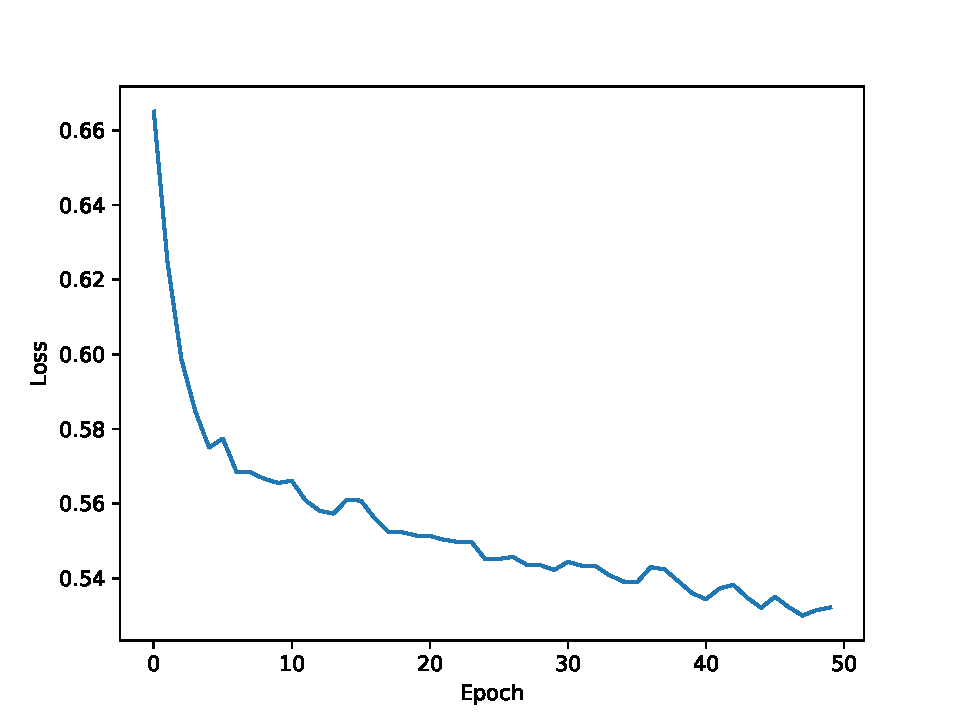
\includegraphics[width=\myWidth]{\imagesPath/MR_train_loss.pdf}
                                    \end{figure}
                            \end{itemize}
                            
                        \item Test dataset:
                            \begin{itemize}
                                \item Accuracy: 0.711
                                \item Recall: 0.418
                                \item F1 score: 0.468
                                \item Loss:
                                    \begin{figure}[H]
                                        \centering
                                        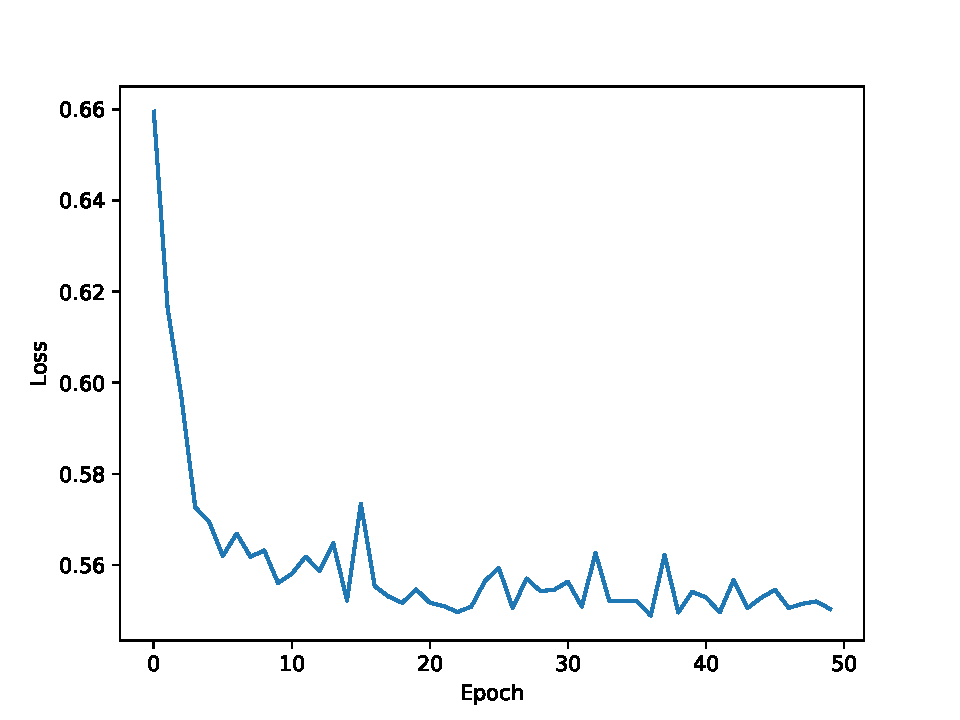
\includegraphics[width=\myWidth]{\imagesPath/MR_test_loss.pdf}
                                    \end{figure}
                            \end{itemize}
                    \end{itemize}
                
                \item Για το dataset \verb|"Semeval2017A"|:
                    \begin{itemize}
                        \item Training dataset:
                            \begin{itemize}
                                \item Accuracy: 0.604
                                \item Recall: 0.516
                                \item F1 score: 0.520
                                \item Loss:
                                    \begin{figure}[H]
                                        \centering
                                        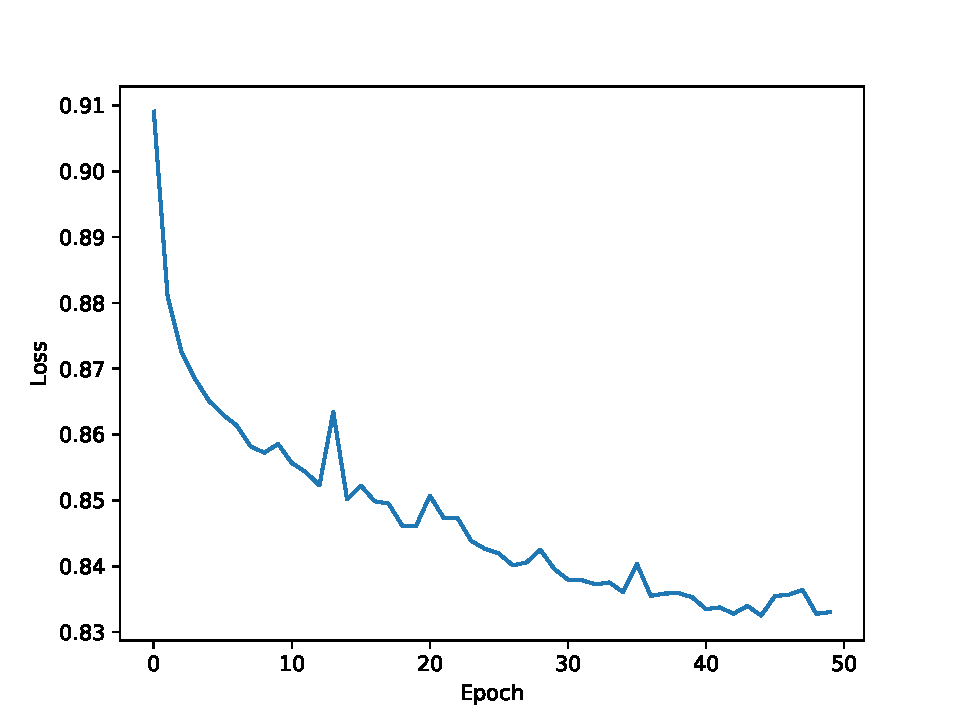
\includegraphics[width=\myWidth]{\imagesPath/Semeval2017A_train_loss.pdf}
                                    \end{figure}
                            \end{itemize}
                            
                        \item Test dataset:
                            \begin{itemize}
                                \item Accuracy: 0.568
                                \item Recall: 0.499
                                \item F1 score: 0.476
                                \item Loss:
                                    \begin{figure}[H]
                                        \centering
                                        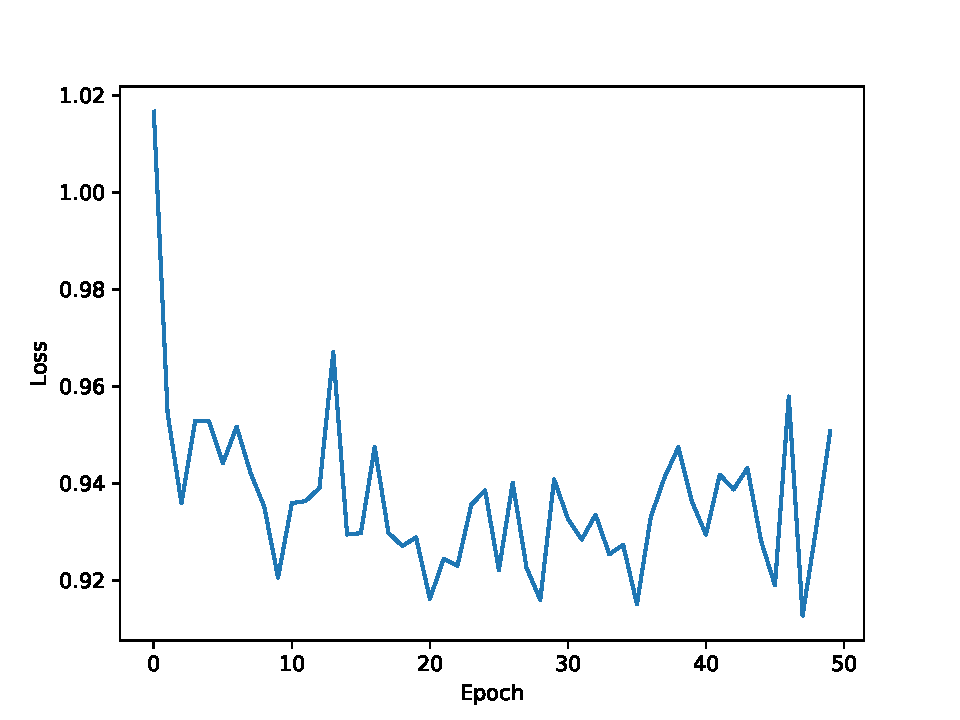
\includegraphics[width=\myWidth]{\imagesPath/Semeval2017A_test_loss.pdf}
                                    \end{figure}
                            \end{itemize}
                    \end{itemize}
            \end{itemize}
            
\end{document}